\documentclass[12pt,a4paper]{article}
\usepackage[utf8]{inputenc}
\usepackage[francais]{babel}
\usepackage[T1]{fontenc}
\usepackage{amsmath}
\usepackage{amsfonts}
\usepackage{amssymb}
\usepackage[left=2cm,right=2cm,top=2cm,bottom=2cm]{geometry}
\usepackage{wasysym}
\usepackage{graphicx}
\usepackage{tikz}
\date{}
\begin{document}
%\begin{large}
\pagenumbering{gobble}  % Pas de numérotation
    \begin{titlepage}

\includegraphics[scale=0.45]{Public/logo_phelma.pdf}\hfill
\includegraphics[scale=0.55]{Public/logo_robotronik.png}
\begin{center}
    \vspace*{2cm}
    \rule{\linewidth}{0.5mm}\\[0.4cm]
    {\huge\bfseries Demande de reconnaissance pour investissement dans des activités associatives\\
    [0.4cm]}\rule{\linewidth}{0.5mm}\\[1.0cm]
    \large{\textsc{Félix Piédallu}}
    \begin{flushright} \large
        2\ieme Année \\
        Filière \textsc{Pns} \\
        Président du \textsc{Club Robotronik}\\
    \end{flushright}
    \vfill

    \large{\today}
\end{center}
\end{titlepage}
     % Fichier de page de titre
\newpage
\pagenumbering{arabic}  % Numérotation de retour !
\part{L'association}
L’Association Robotronik (association loi 1991) a été créé en 2008 résultant de la fusion de PG Robotik et du Club Électronique.
La vocation de l'association est la promotion de la robotique et des  domaines qui y sont liés. Le club encadre des projets personnels et participe chaque année à la Coupe de France de Robotique qui rassemble chaque année quelques 200 équipes d’étudiants et de passionnés. Il participe également à l'organisation de quelques événements à Phelma (Fête de la Science, Coupe  FIRST).
\part{Mon rôle au sein de l’association}

Au sein de l'association Robotronik j'ai le rôle de Chef de Projet : je suis chargé de mener les projets au sein de l'association et en particulier  le projet « Coupe de France ». J'anime donc l'équipe qui doit réaliser les deux robots qui doivent participer à la coupe. J'ai donc un rôle managérial : étant garant de l'avancement des projets il me faut diriger une équipe qui n'a pas d'obligation contractuelle car bénévole, ce qui peut parfois causer un certain relâchement quant au travail fourni. Je dois donc rester vigilant à maintenir la motivation générale (sans pour autant exiger un engagement total des membres). J'ai également un rôle organisationnel : il me faut répartir dans le temps et manière optimisée les différentes tâches à effectuer et les distribuer aux membres en fonctions des compétences et affinités de chacun. Le but du club étant aussi d'apprendre il faut que je veille également à ce qu'un membre ne soit pas cloisonné dans ses tâches et que chacun puisse apprendre des autres. Cette répartition se fait en concertation avec les responsables des différents domaines techniques présents au club (Mécanique, Électronique et Informatique). Je dois donc être relativement compétant dans  chacun des trois domaines car je suis souvent amené à y intervenir pour donner une cohérence au développement parallèle des composantes des robots.

\part{Description de mes objectifs et objet de ma demande de reconnaissance}
Mes objectifs sont bien évidemment d'avoir des robots les plus performants possible pour pouvoir faire bonne figure à la coupe. Pour cela il a été décidé trois changements techniques : le passage à des batteries plus performantes, le changement de capteurs de proximité qui ont été responsables de quelques problèmes l'an dernier et l'utilisation de nouveaux microcontrôleurs fournis par ST. Je vais donc encadrer au mieux ces aspects là qui vont représenter un investissement plus important en temps et ressources. Il va également falloir s’adapter aux nouvelles règles pour la prochaine compétition ce qui va nous demander également de développer des solutions spécifiques. Par exemple nous évoquons  la possibilité d'utiliser des chenilles pour pouvoir monter les marches présentes cette année sur la table de jeu. Nous aurons donc à modifier une partie importante du programme gérant le déplacement des robots en tenant compte de ce qui a été fait au niveau mécanique.  J’interviens donc ici afin de gérer au mieux la cohérence de deux parties qui ne seront pas réalisées par les mêmes personnes.
\paragraph{} Ma demande s'appuie donc d'une part sur le temps important que devrais consacrer (et que j'ai déjà consacré) au club et d'autre part sur les connaissances que je pourrai retirer de cette expérience et qui peuvent se substituer à certains cours. Cet aspect est détaillé ci-après.
\part{Apport de l'investissement par rapport au futur métier d'ingénieur}
Ces responsabilités au sein du club vont pouvoir me faire découvrir les aspects gestion d'équipe, développement d'un produit, gestion des délais et respect de cahier des charges … Ce sont des compétences qui peuvent être attendues de la part d'un ingénieur. Cela me permettra également d'avoir une très bonne expérience du travail en équipe et de sa gestion si je suis amené, par le futur, à diriger une équipe et, même si ce n'est pas le cas, connaître les difficultés qui y sont liées reste très formateur ne serait-ce que pour faciliter la communication avec un potentiel futur dirigeant. Les délais sont évidement également un aspect rencontré dans le métier d'ingénieur (comme beaucoup d'autre par ailleurs) et savoir les maîtriser est un atout non négligeable. Pour finir le développement de nouveaux produits répondants à certaines attentes,  comme nous serons amenés à faire au club, s'apparente au domaine de la R\&D qui m'attire fortement.

\part{Échéancier de mise en œuvre de l'action et estimation du temps nécessaire}
Nous avons décidé de nous donner comme échéancier la pré-coupe de Lyon qui a lieu en mars. Ceci afin de nous laisser le temps d'améliorer et de paramétrer les robots en fonction des résultats que nous y aurons obtenus.
L'échéancier se subdivise naturellement en trois sous catégories (en ce qui concerne la partie technique) qui sont les composantes du club : mécanique, électronique et informatique. Sachant que la mécanique influe sur le dimensionnement de l'électronique  et que l'informatique dépend des choix mécaniques et électroniques. Cependant en électronique et informatique de nombreuses parties peuvent commencer à être abordées avant la mécanique car elles n'en dépendent pas (ou pas dans un premier temps). Il a donc été décidé que la modélisation de la mécanique se terminerait en novembre pour pouvoir terminer le dimensionnement de l'électronique en janvier et démarrer la programmation qui dépend des choix faits dans la même période (partie stratégie sur le Gantt). La réalisation complète der robots (placée en partie mécanique et prenant fin en mars) se fera de front avec la réalisation des différentes cartes électroniques de manière à les intégrer au fur et à mesure.
\begin{figure}[hh]
    \begin{center}
        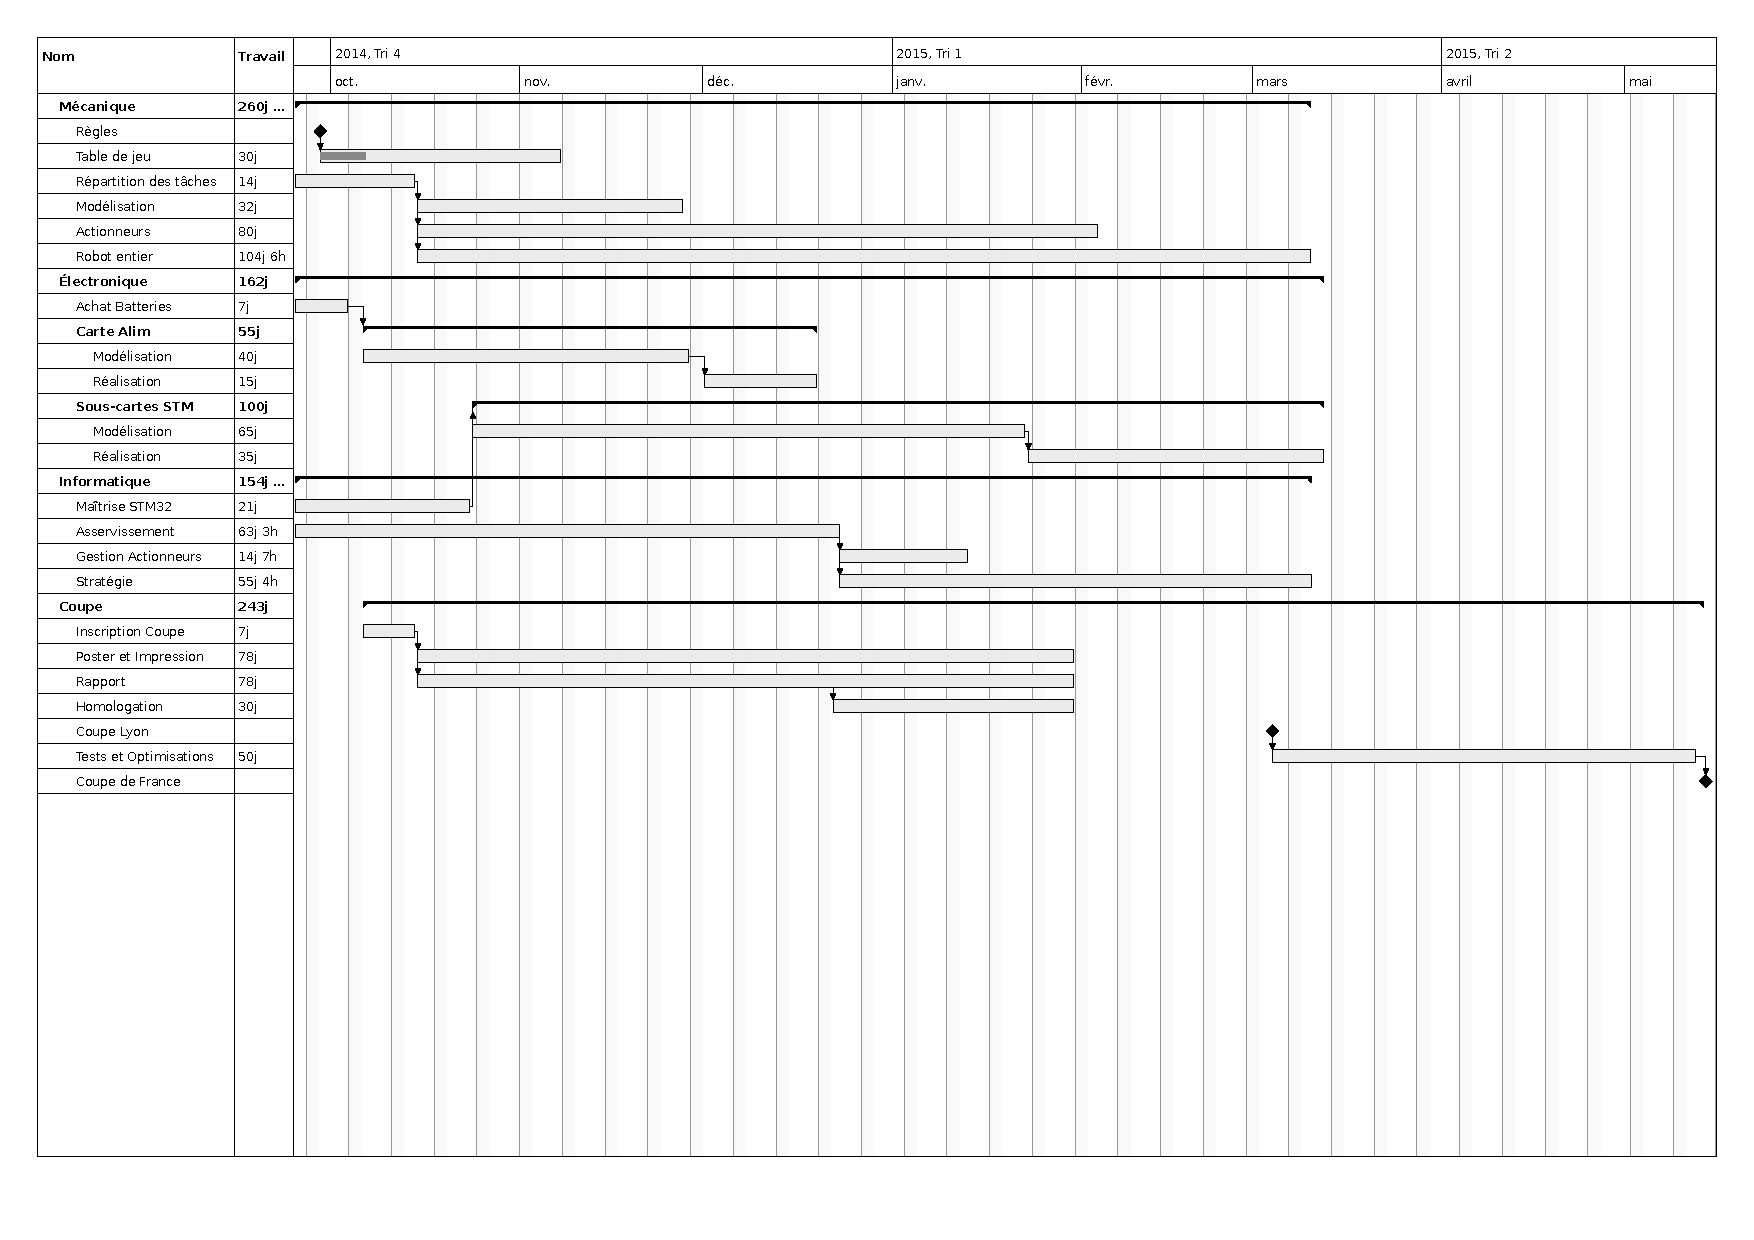
\includegraphics[trim=27px 215px 17px 33px,clip=true , width=\textwidth]{Public/GanttRobo.pdf}
        \caption{Gantt du Club Robotronik}
    \end{center}
\end{figure}
\paragraph{}
Tout ceci demande un minimum d'engagement c'est pourquoi le temps que je consacre au club est compris entre 6 et 7 heures (comprenant un minimum de 5h en présentiel au club), ceci en prenant en compte les samedis robotique qui auront lieu quand l'échéance de la coupe arrivera.
Le cumul sur l'année du nombre d'heures sera donc approximativement de 250h.



\part{Périodes et contenus livrables}
La pré-coupe de Lyon (en mars) constitue l'échéancier ou les robots devront être fonctionnels bien que largement optimisables pour la coupe de France. Les robots devront en effet être entièrement montés. Au mois de mai les robots serons entièrement configurés et optimisés et pourrons être considérés comme « produit fini ». Cependant  un ensemble de dates peuvent aussi constituer des points de suivis à respecter : la table de jeu, par exemple devra être terminée début Novembre afin de permettre les différents tests qui suivrons. Une première modélisation de robot est prévue pour fin décembre, ce qui permettra de passer à la réalisation et de commander à nos sponsors la découpe des éléments nécessaires à la carrosserie. En ce qui concerne la carte de gestion des nouvelle batteries, qui n'est pas dépendante des choix mécaniques, elle sera « livrable » mi-décembre. De cette manière nous pourrons réaliser des tests en conditions réelles (et non pas  avec une alimentation branchée sur le secteur ou avec nos anciennes batteries).
%\end{large}
\appendix
\newpage
\begin{center}
\vspace*{10cm}
{\huge\bfseries Annexes\\
[0.4cm]}\rule{\linewidth}{0.5mm}
\end{center}

\newpage
\section{Organigramme du Club Robotronik}

\vspace*{3cm}
\begin{center}
\begin{tikzpicture}
\tikzstyle{bureau}=[rectangle, minimum height=1.8em,fill=yellow!30,text=black]
\tikzstyle{respo}=[rectangle, minimum height=1.8em,fill=blue!20,text=black]
    \node[bureau] (Prez) at (0,0) {Félix Piédallu, Président};
    \node[bureau] (Trez) at (-5,-1) {Ojeme Ikhalo, Trésorier};
    \node[bureau] (Secr) at (+5,-1) {Florence André, Secrétaire};
    \node[respo] (Chef) at (+0,-2.3) {Johan Lafon, Chef de Projet};
    \node[respo] (Elec) at (-5,-4) {Robin Moussu, Respo Électronique};
    \node[respo] (Info) at (+0,-5) {Robin Moussu, Respo Informatique};
    \node[respo] (Meca) at (+5,-4) {Florence André, Respo Mécanique};
    
    
\tikzstyle{ens}=[<->,dotted,very thick,>=latex]
\tikzstyle{sup}=[<->,dotted,very thick,>=latex]
    \draw[ens] (Chef) -- (Meca);
    \draw[ens] (Chef) -- (Info);
    \draw[ens] (Chef) -- (Elec);
    
    \draw[sup] (Trez) -- (Prez);
    \draw[sup] (Secr) -- (Prez);
    
    \draw[sup] (Prez) -- (Chef);
    \draw[sup] (Trez) -- (Chef);
    \draw[sup] (Secr) -- (Chef);
\end{tikzpicture}
\end{center}
\vspace*{7cm}
\begin{figure}[h]
    \begin{flushright}
        Le Président, Félix Piédallu, le 9 Octobre 2014,\\
        
\includegraphics[width=100px]{Public/SignaturePresident}
    \end{flushright}
\end{figure}


\end{document}
